\section{Lucky Patcher} \label{section:luckypatcher-explain}
%START TEXT INPUT


%START TEXT INPUT

%
reason lucky ptcher is taken exremely popular and easy(no technical knowdlege except root but apps can be traded)

main goal is to circumvent license verification, app should behave as it is legally aquired in app store, by user hence work normally, full features

most common way client-server license verification, app gathers info and sends to server, server checks info and depending on this sends response, finally app acts according to response code

since server is not accessible and man-in-the-middle has to break encryption, like spoofing, which is difficult (encryption in general), has to work in application

effective, popular, vielseitig (viel internet -see- quelle)
high damage potential since popular, automated and general use by non professional

\cite{munteanLicense}
%

written by ChelpuS

for this master's thesis the version 5.9.5
written bei chelphus
requires root and busybox, an application which provides standard UNIX tools for Android\cite{busyboxApp}
apply patches:
- Remove license check in premium apps (used to crack DRM)
- remove ads
-Customize and restrict permissions and activities
-Create a modified app (means an APK file to install the app with a patch already applied)

\begin{figure}[h]
    \centering
    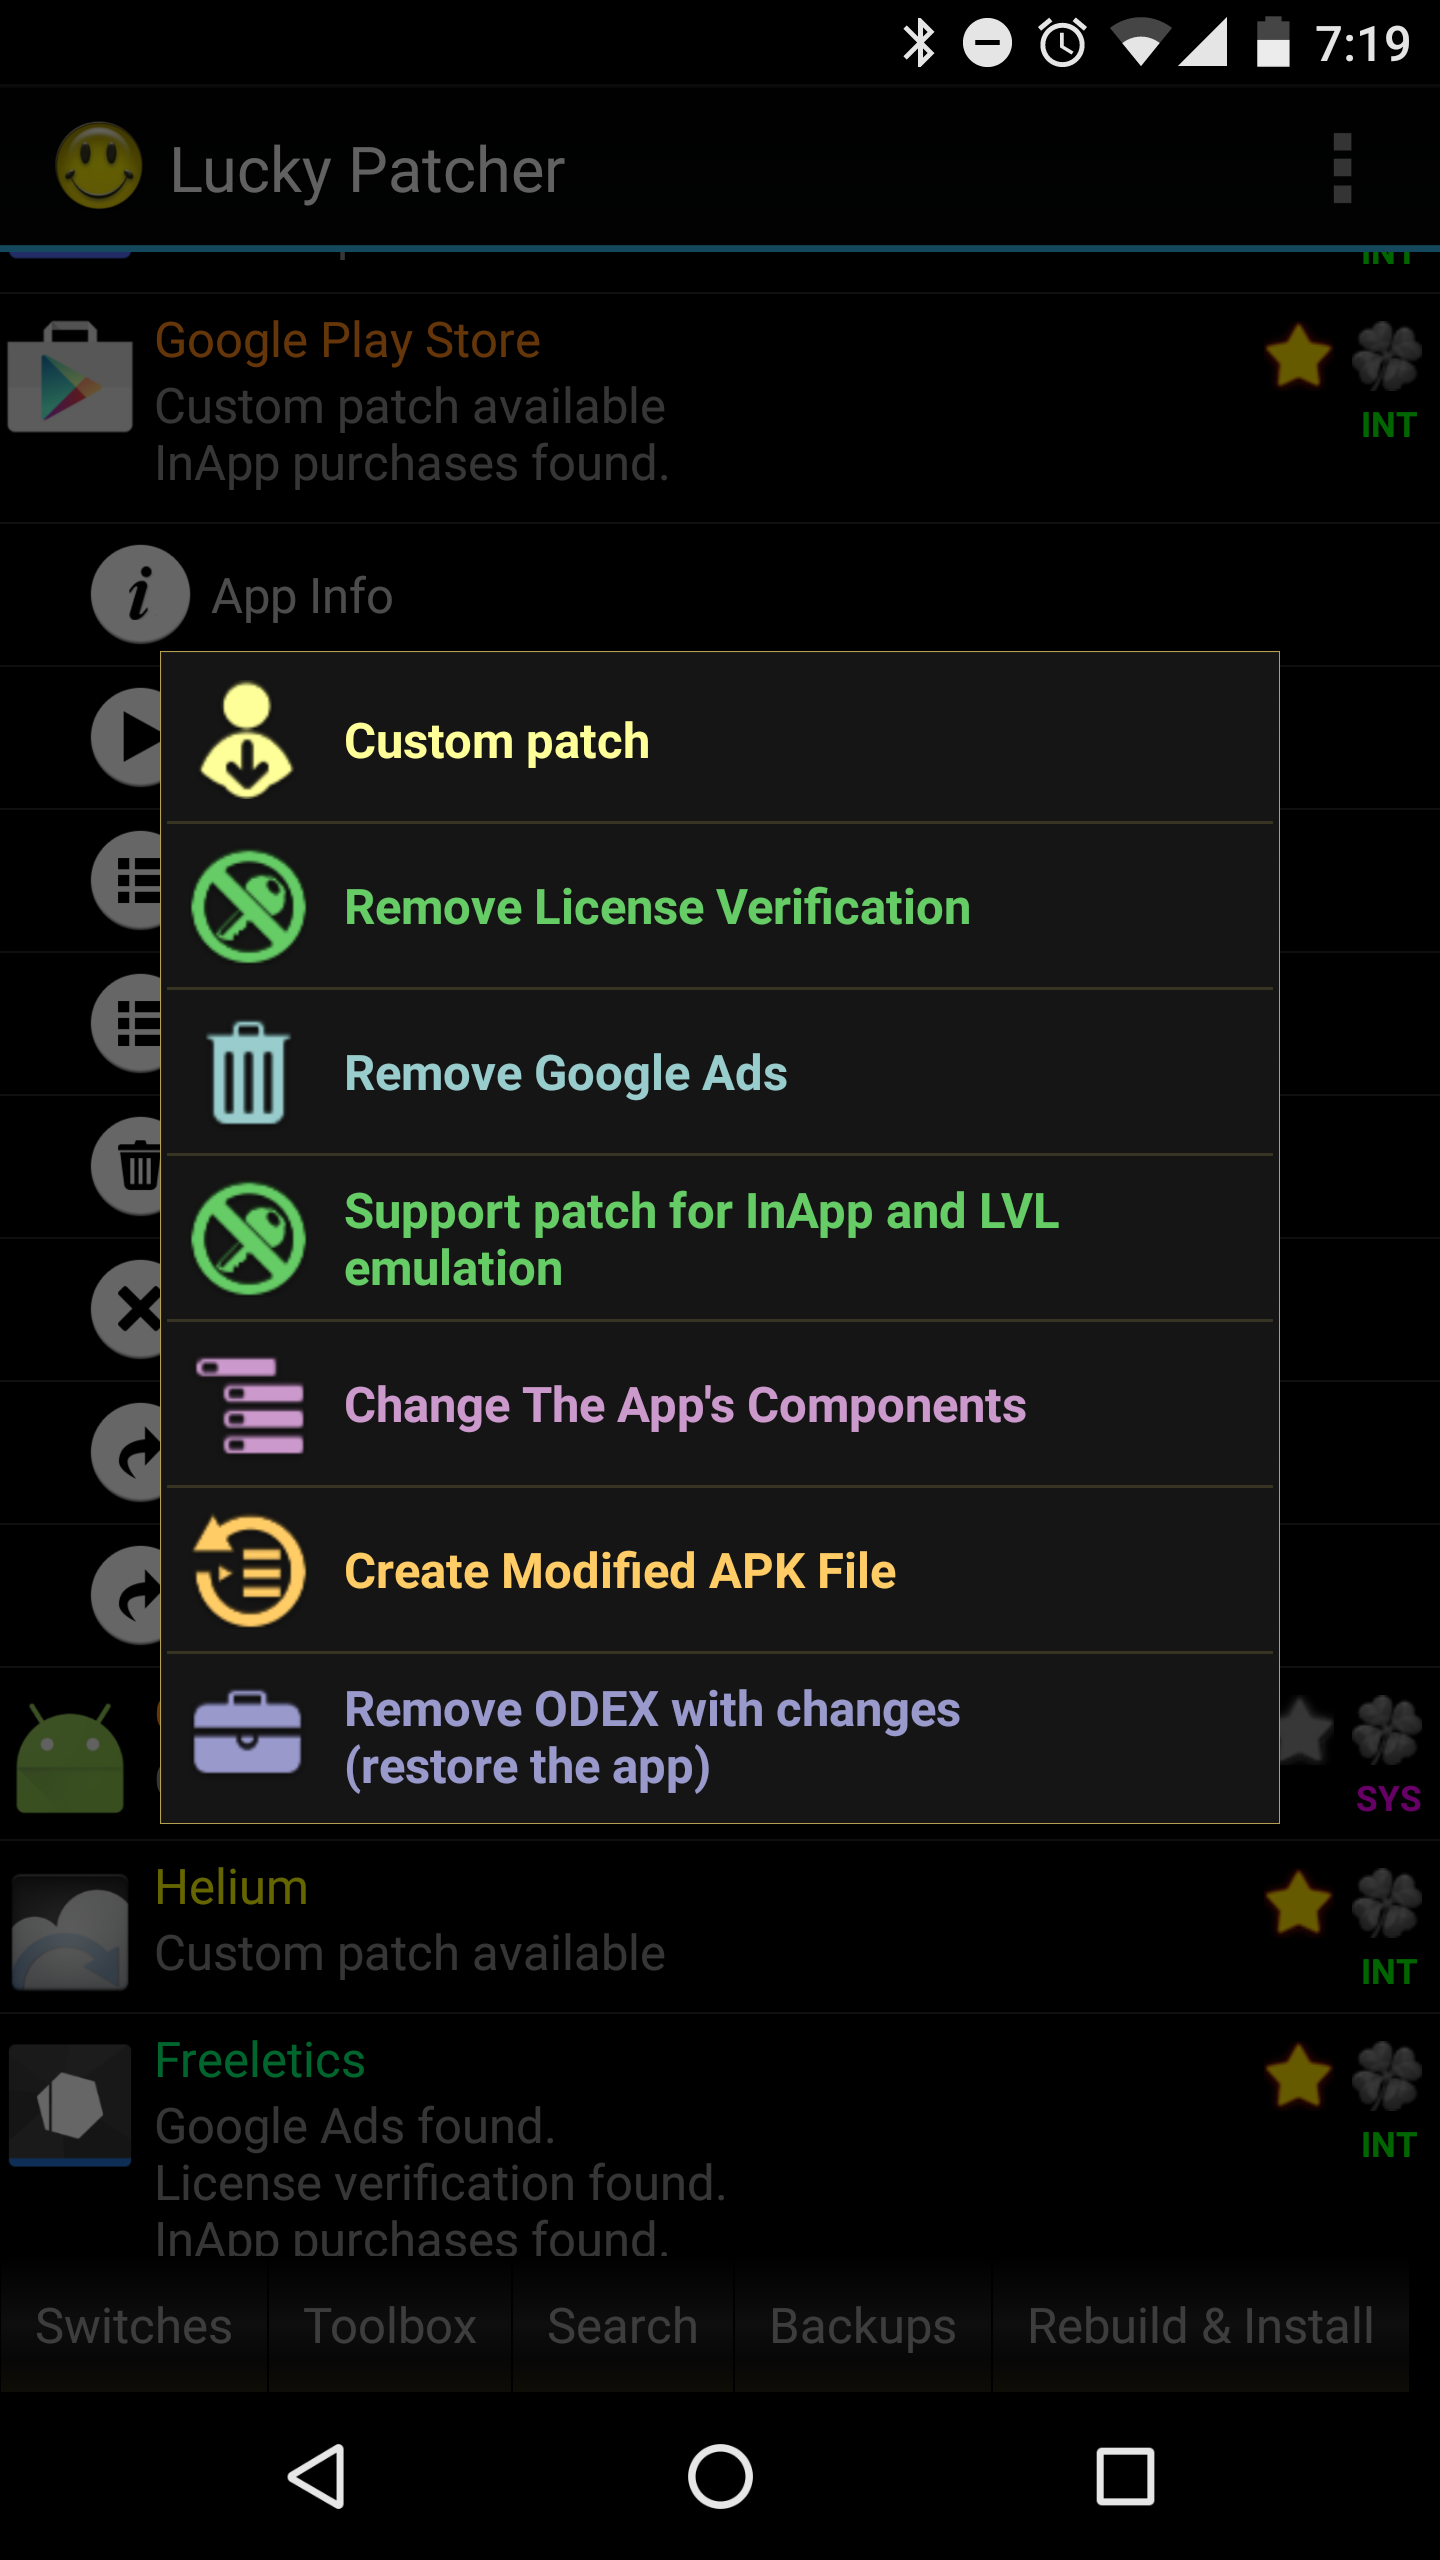
\includegraphics[width=0.3\textwidth]{data/luckyFeatures.png}
    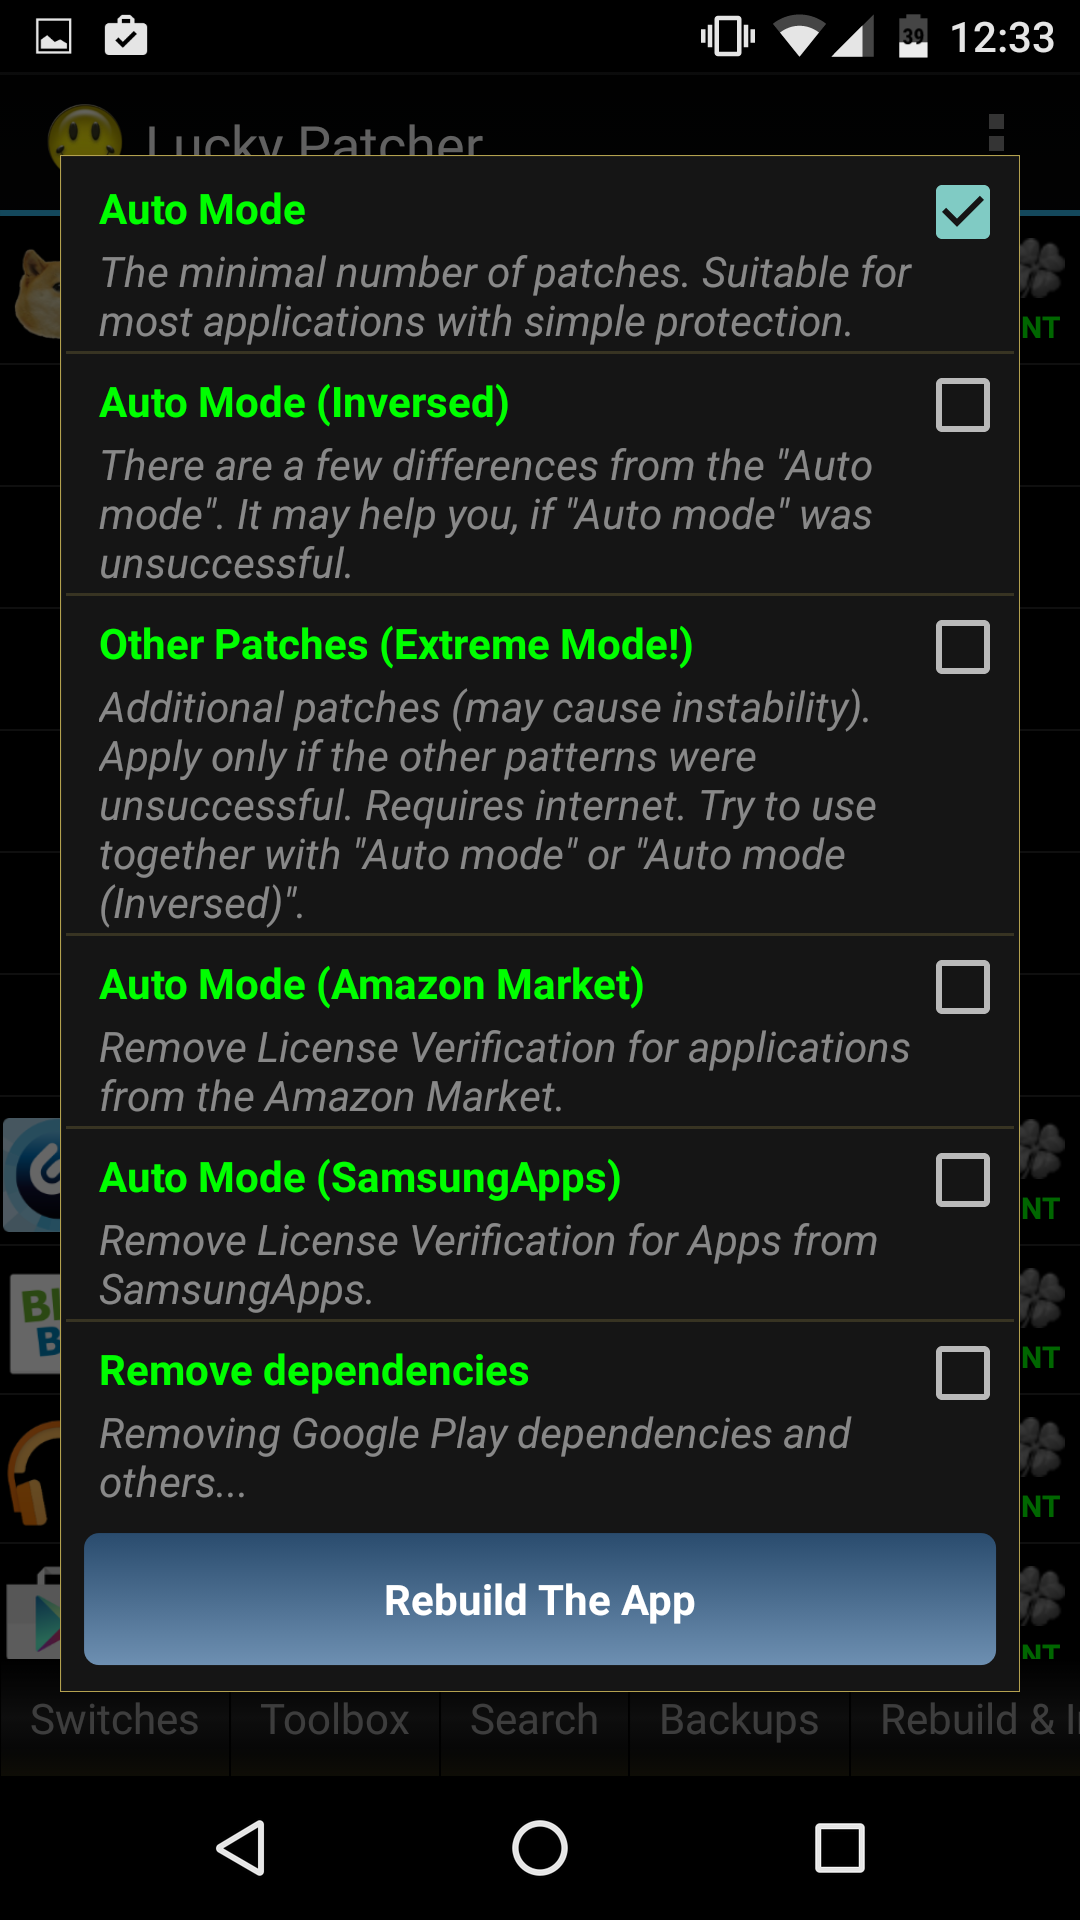
\includegraphics[width=0.3\textwidth]{data/luckyModi.png}
    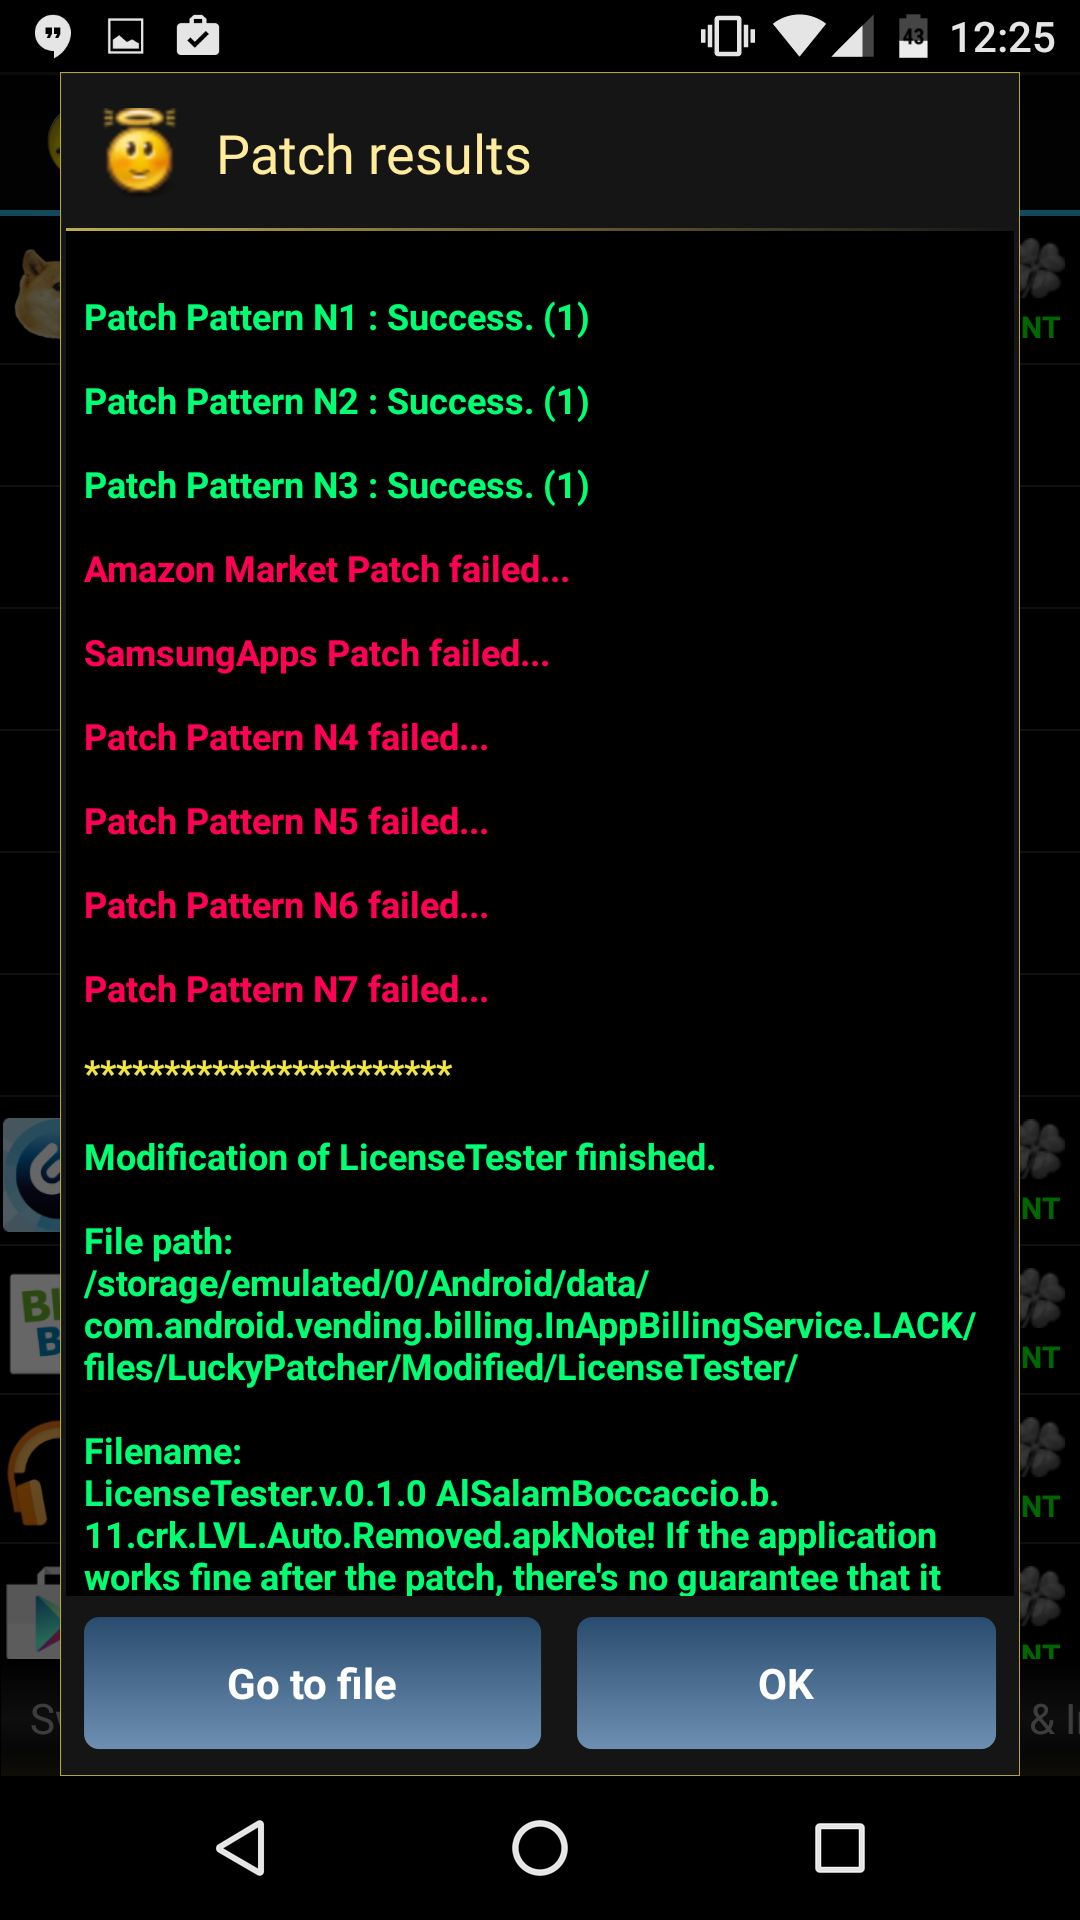
\includegraphics[width=0.3\textwidth]{data/luckyPatching.png}
    \caption{c}{Left: Features offered Lucky Patcher
    Middle: Variants to crack license verification
    Right: Result after patching}
    \label{fig:luckyScreen}
\end{figure}

not 100percent warranty that patching works due to modified libraries


erklären wie man ihn gestestet hat, woher die apps, nachgefragt ob ok etc

Lucky Patcher is described as following on the offical webpage: "Lucky Patcher is a great Android tool to remove ads, modify apps permissions, backup and restore apps, bypass premium applications license verification, and more. To use all features, you need a rooted device." \cite{luckyPatcherOfficial}

install apk from playstore -see- have root -see- open lucky -see- chose mode


this thesis focuses on the removing of licensing check, angewendet auf verschiedene apps aus den jeweiligen stores
